\section{Results and Discussion}
\label{sec:res-disc}

The evaluation of noise levels and harmonic distortion is vital in assessing the performance and reliability of electronic systems. In the context of the cytometer platform, accurate measurements of noise and harmonics provide insights into the system's ability to maintain signal integrity and mitigate external disturbances. This section presents the results of comprehensive noise and harmonic measurements conducted on the platform, revealing its noise reduction capabilities and harmonic attenuation performance.

% --- Harmonics ---

Thorough testing of the cytometer platform required the inclusion of MR sensors to detect and measure changes in magnetic fields. To generate the necessary magnetic field for testing, a system comprising two coils and a driver power op-amp was utilized. The coils, arranged in a Helmholtz coil pair configuration, created a nearly uniform magnetic field, providing a controlled environment for the MR sensors. This allowed for accurate performance testing and validation of the platform's functionality.

One important performance test conducted using this system was the evaluation of harmonic distortion, depicted in Figure \ref{fig:harmonics}. Harmonics can introduce noise and distort the waveform shape, potentially compromising signal quality. Managing harmonic distortion is crucial for maintaining signal integrity in sensitive applications like the cytometer platform. 

The test involved two experiments, each utilizing a magnetic field with different frequencies. The blue trace represents the $\mathrm{1~kHz}$ frequency, while the green trace represents the $\mathrm{10~kHz}$ frequency.

\begin{figure}[!ht]
    \centering
    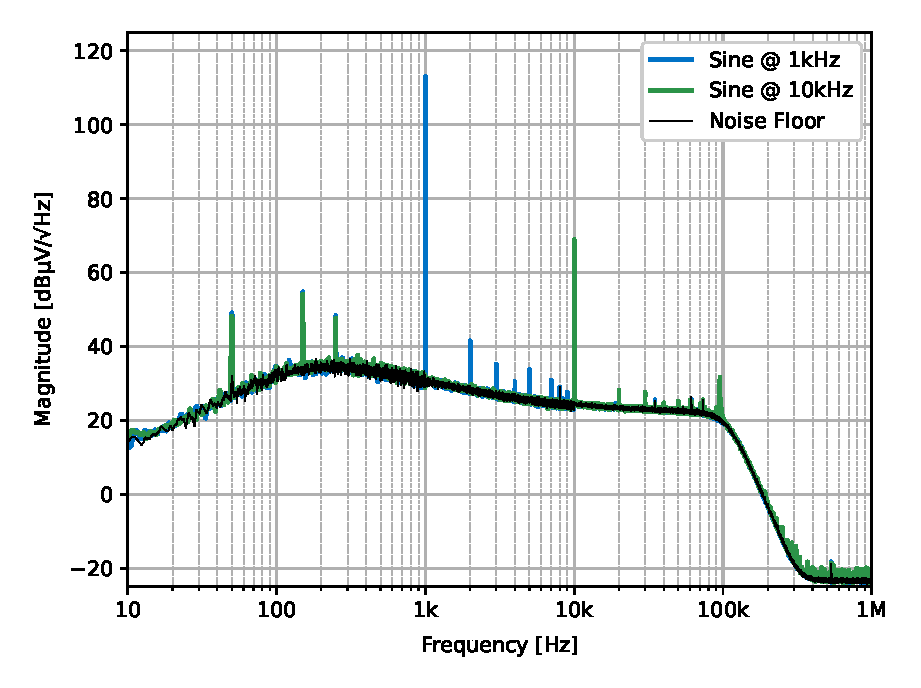
\includegraphics[width=.475\textwidth]{figs/harmonics.eps}
    \caption{Magnetic field measurements.}
    \label{fig:harmonics}
\end{figure}

The results of the harmonic performance analysis, shown in Figure \ref{fig:harmonics}, demonstrated impressive attenuation of approximately $\mathrm{70~dB}$ between the 2\textsuperscript{nd} and 1\textsuperscript{st} harmonics at a fundamental frequency of $\mathrm{1~kHz}$. This high level of attenuation ensures precise signal reproduction and minimal distortion. Although the attenuation was slightly lower at $\mathrm{10~kHz}$ due to the frequency response characteristics of the coil driver, the system effectively suppressed undesired harmonic components, preserving signal integrity.

% --- Noise ---

The ultra-low noise interface circuitry plays a crucial role in enhancing the performance of MR sensors used in the cytometer platform. By minimizing noise-induced fluctuations, the accuracy of magnetic field measurements is preserved, ensuring precise detection of magnetic field changes. The interface circuitry effectively mitigates noise contributions from various sources, including biasing, addressing, amplification, and output multiplexing. Through careful design and optimization, the SNR is improved, leading to enhanced accuracy and reliability of measurements. The noise reduction achieved in this work surpasses the previous interface version, as depicted in Figure \ref{fig:noise}, even with the introduction of additional features such as sensor addressing and output multiplexing. The successful implementation of a different type of reference in the new platform contributed to superior noise performance.

\begin{figure}[!ht]
    \centering
    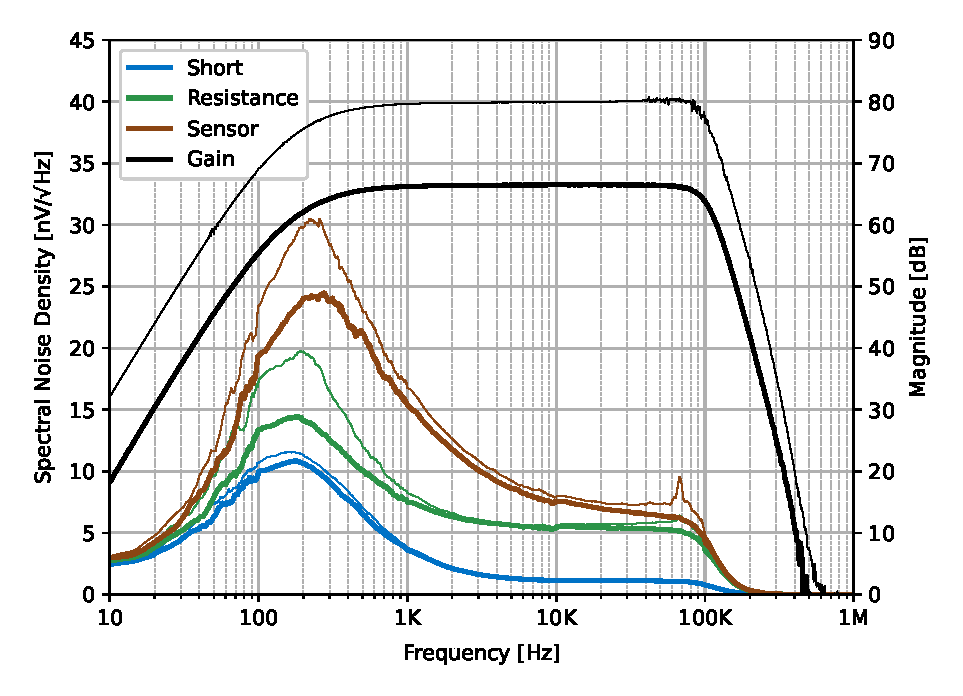
\includegraphics[width=.475\textwidth]{figs/noise.eps}
    \caption{Noise measurements -- Comparison between the old platform and the one presented in this work.}
    \label{fig:noise}
\end{figure}

Figure \ref{fig:noise} displays the noise measurements for both platforms. The thicker line represents the interface developed in this work, while the thinner line represents the previous interface. The graph clearly shows a reduction in overall flicker noise in the new interface. Additionally, the gain has been decreased to accommodate the input voltage limitation of the ADCs.

Overall, the strategies and circuitry optimizations employed in the interface circuitry have resulted in a more robust and reliable system, enabling accurate measurements in the presence of external noise sources.

\begin{figure*}[!htbp]
    \centering
    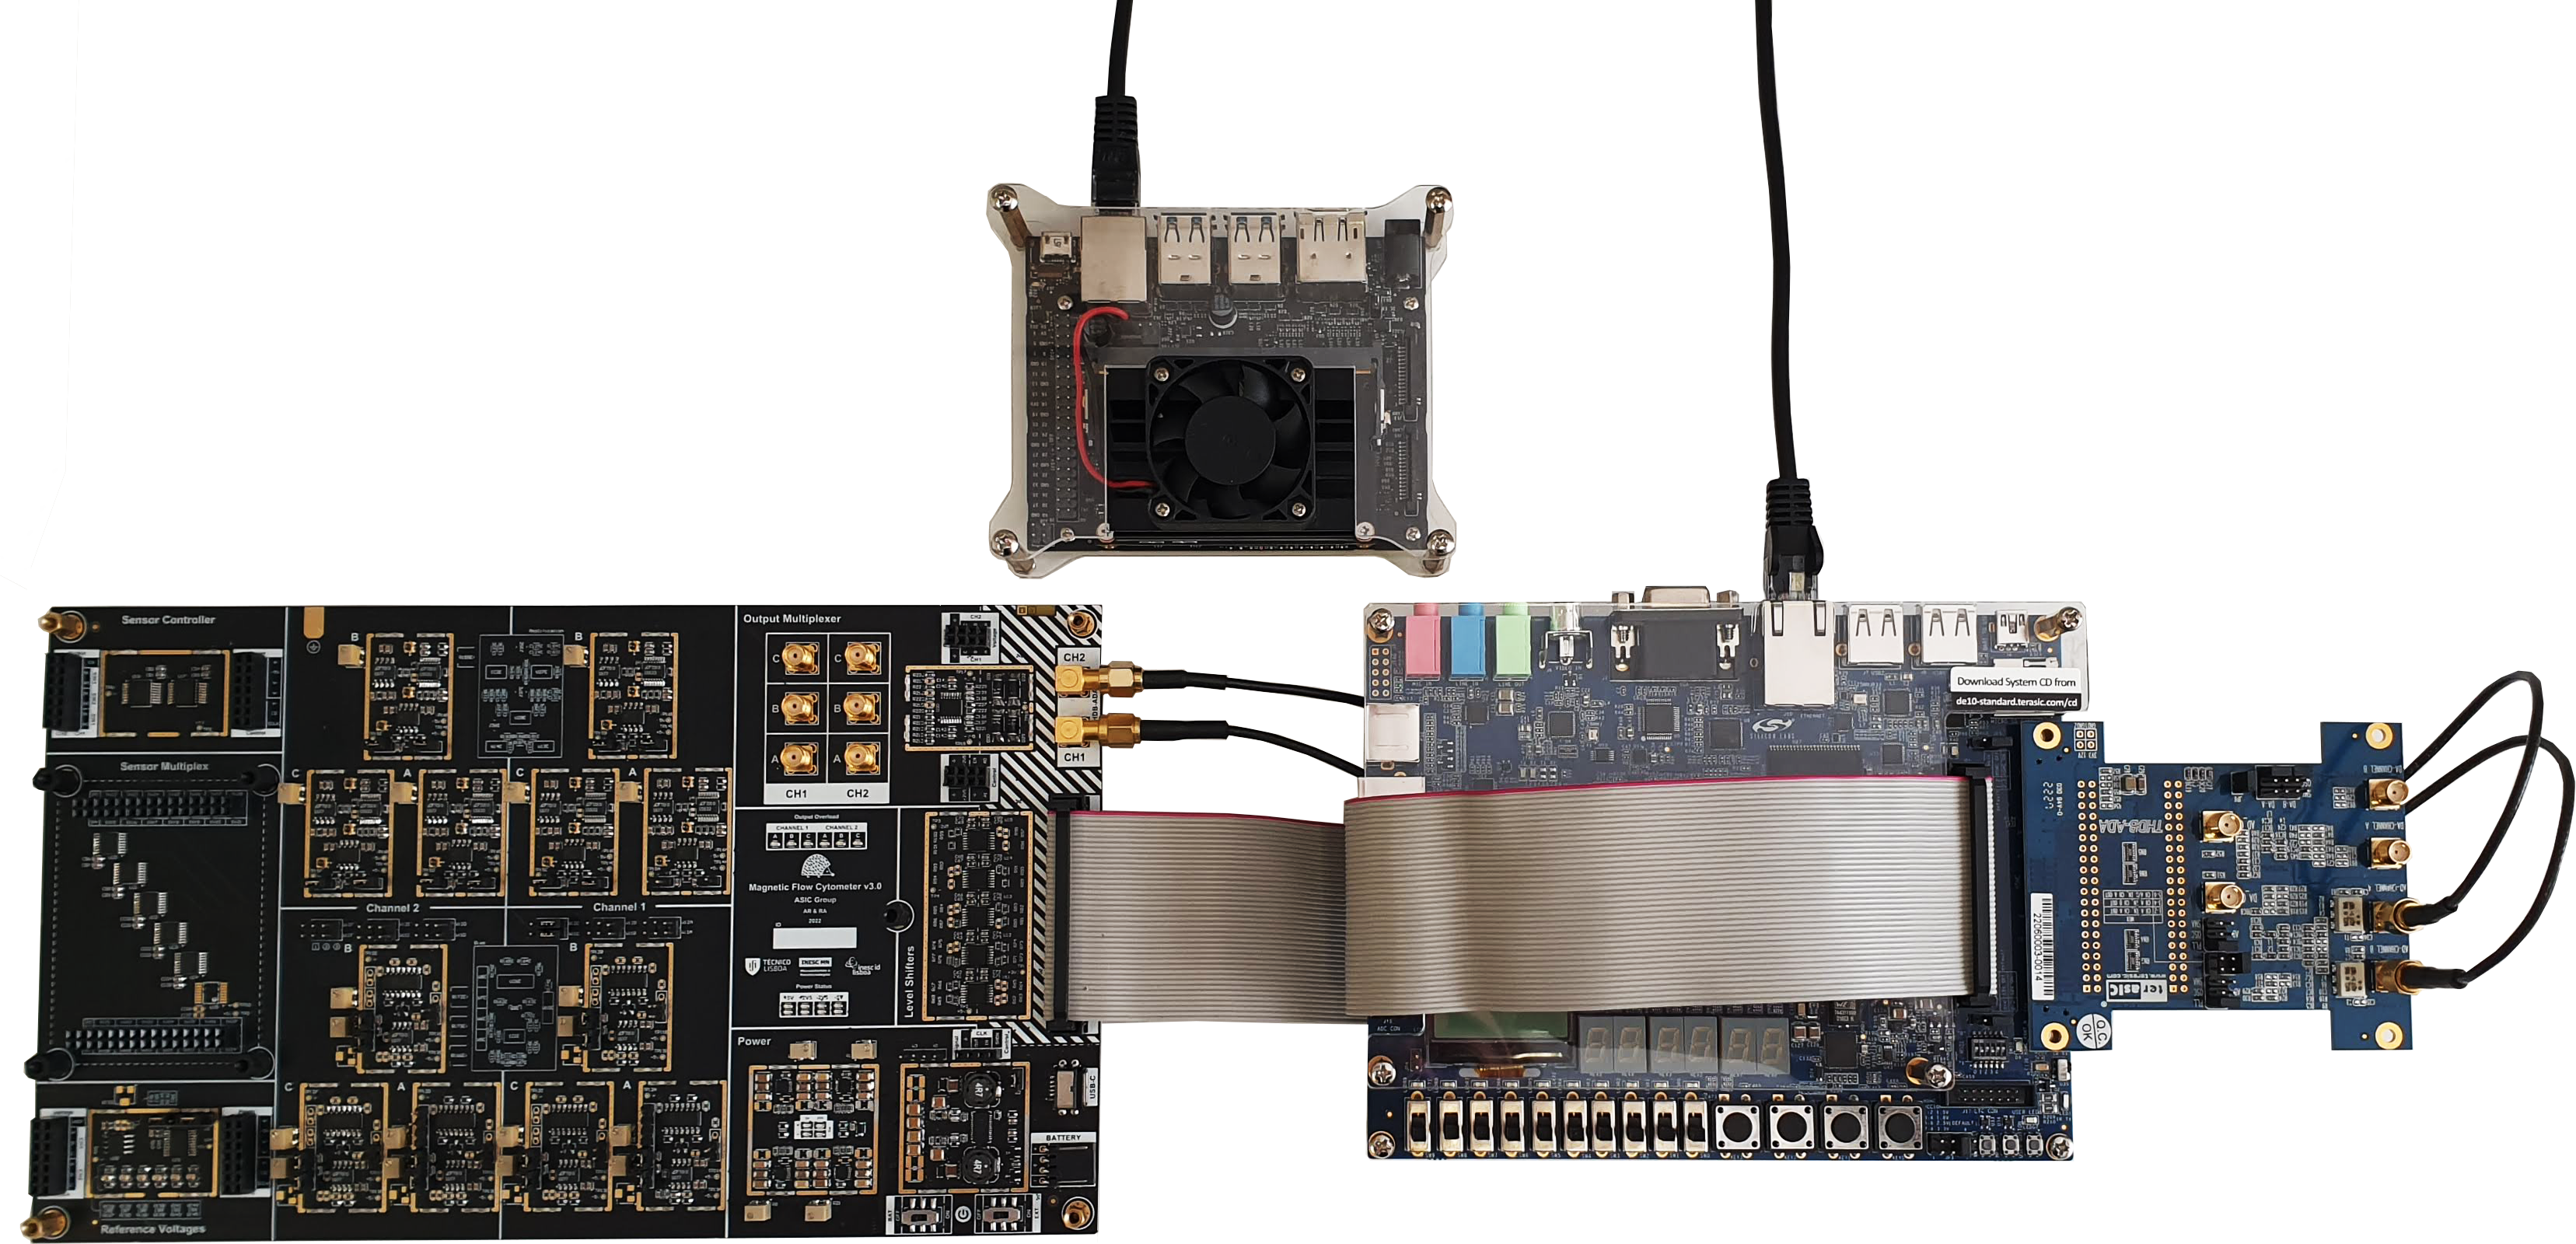
\includegraphics[width=.9\textwidth]{figs/system.png}
    \caption{MFC System.}
    \label{fig:mfc}
\end{figure*}

Figure \ref{fig:mfc} shows the different boards that make up the cytometer system. The left PCB, distinguished by its black solder mask, represents the cytometer platform that was developed as part of the work being described. On the right side, the blue PCB represents the FPGA (DE-10 Standard) and the acquisition board (THDB-ADA). At the top of the figure, the compact computer (Jetson-Nano) serves as the platform that will execute a real-time machine-learning algorithm.